\section{Ondas. El Sonido}

\subsection{Cinemática de la Ondas}

\begin{enumerate}
	\item \textsc{\textbf{Movimiento Periódico}}: Es un movimiento que se \textbf{repite} cada cierto intervalo de \textbf{tiempo}, por ejemplo, el movimiento de los planetas, el péndulo de un reloj o un muelle que vibra.
	\item \textsc{\textbf{Movimiento Oscilatorio}}: Es un movimiento que tiene un cuerpo que se \textbf{desplaza} a un lado y a otro de su posición de \textbf{equilibrio}, de forma \textbf{periódica}. Por ejemplo, el péndulo de un reloj o un muelle que vibra.
	\item \textsc{\textbf{Movimiento Vibratorio}}: Es un movimiento \textbf{oscilatorio} con una \textbf{trayectoria rectilínea}. Por ejemplo, un muelle que se comprime.
\end{enumerate}

En todos los movimientos periódicos denominamos:

\begin{enumerate}
	\item \textbf{Periodo} ($T$): Intervalo de \textbf{tiempo} que tarda un cuerpo en \textbf{repetir} su movimiento. Medido en segundos (\unit{\second}).
	\item \textbf{Frecuencia} ($f$): Número de \textbf{repeticiones} que realiza un cuerpo en un \textbf{segundo}. Medida en Hercios (\unit{\hertz}) o la inversa del segundo (\unit{\per\second}).
\end{enumerate}
	
Ambas \textbf{magnitudes} están \textbf{relacionadas} por la expresión:

\begin{equation}
f = \frac{1}{T} \Longleftrightarrow T = \frac{1}{f}
\end{equation}

\subsection{Movimiento Armónico Simple}

El movimiento armónico simple es el movimiento que tienen los cuerpos que se mueven por acción de una fuerza restauradora proporcional a la distancia que separa al cuerpo de su posición de equilibrio. Viene dada por la ecuación:

\begin{equation}\label{ONDASS_MVAS}
    x(t) = A \cdot \sin(\omega \cdot t + \varphi_0)
\end{equation}

Donde:
\begin{enumerate}
    \item $x(t)$: Elongación (\unit{m})
    \item $A$: Amplitud (\unit{m})
    \item $\omega$: Frecuencia o velocidad angular (\unit{\radian\per\second})
    \item $\varphi_0$: Fase inicial o desfase (\unit{\radian})
    \item $\omega \cdot t + \varphi_0$: Fase (\unit{\radian})
\end{enumerate}

\subsubsection{Representación Gráfica del MAS}

\begin{figure}[h!]
    \centering
    \begin{tikzpicture}[scale=1.1]
        % Parámetros
        \def\A{1}
        \def\T{4}
        \def\w{2*pi/\T}

        % Ejes
        \draw[->, thick] (0,-1) -- (0,1) node[above] {};
        \draw[->, thick] (-0.2,0) -- (10,0) node[right] {$t$};

        % Marca de amplitud A
        \draw[thick] (-0.15,\A) -- (0.15,\A);
        \node[left] at (0,\A) {$A$};

        % Onda MAS
        \draw[very thick, red]
        plot[domain=0:10, samples=200]
        (\x,{\A*sin(\w*\x r)});

        % Marcas de T y 2T
        \draw[thick] (\T,0.15) -- (\T,-0.15);
        \node[below] at (\T,-0.2) {$T$};

        \draw[thick] (2*\T,0.15) -- (2*\T,-0.15);
        \node[below] at (2*\T,-0.2) {$2T$};

        % Línea vertical discontinua en T
        \draw[dashed] (\T,-1) -- (\T,1);

        % Flecha periodo
        \draw[<->, thick] (0,-1) -- (\T,-1);
        \node[below] at (\T/2,-1) {$T = \dfrac{2\pi}{\omega}$};
    \end{tikzpicture}
    \caption{Representación gráfica del MAS de la amplitud con respecto del tiempo}
    \label{ONDASS_GRAFICAMAS}
\end{figure}